\documentclass{report}


\usepackage[T1]{fontenc}
\usepackage[utf8]{inputenc}
\usepackage{amsmath}


\usepackage{enumerate}

\usepackage{graphicx}
\usepackage{fancyhdr}
\usepackage{lettrine}
\usepackage{hyperref}
\usepackage{subcaption}
\usepackage{tikz}
\usepackage{cite}
\usepackage{listings}
\usepackage[nottoc, numbib]{tocbibind}
\usepackage[ngerman]{babel}
\usepackage[Glenn]{fncychap}
\usepackage{trfsigns}
\usepackage{parskip}
\usepackage{microtype}


\usetikzlibrary{shapes}
    \usetikzlibrary{arrows}
    \usetikzlibrary{arrows.meta,topaths}
    \usetikzlibrary{bending}
    \usetikzlibrary{calc}
\title{Elektrotechnik 1 Praktikum 1}


\usepackage[
  includehead,
  headheight = 17mm,
  footskip = \dimexpr\headsep+\ht\strutbox\relax,
  tmargin = 0mm,
  bmargin = \dimexpr17mm+2\ht\strutbox\relax,
]{geometry}

\usepackage{anyfontsize}
\usepackage{float}
\usepackage{xcolor}

\definecolor{DarkGreenBlue}{HTML}{264653}
\definecolor{LightGreenBlue}{HTML}{2A9D8F}
\definecolor{LightOrange}{HTML}{E9C46A}
\definecolor{DarkOrange}{HTML}{F4A261}
\definecolor{RedOrange}{HTML}{E76F51}
\definecolor{BrightRed}{HTML}{D62828}
\definecolor{DeepBlue}{HTML}{003049}

\lstdefinestyle{code}{
    backgroundcolor=\color{backcolour},
    commentstyle=\color{codegreen},
    keywordstyle=\color{magenta},
    numberstyle=\tiny\color{codegray},
    stringstyle=\color{codepurple},
    basicstyle=\ttfamily\footnotesize,
    breakatwhitespace=false,
    breaklines=true,
    captionpos=b,
    keepspaces=true,
    numbers=left,
    numbersep=5pt,
    showspaces=false,
    showstringspaces=false,
    showtabs=false,
    tabsize=2
}

\definecolor{codegreen}{rgb}{0,0.6,0}
\definecolor{codegray}{rgb}{0.5,0.5,0.5}
\definecolor{codepurple}{rgb}{0.502,0.502,0.0}
\definecolor{backcolour}{rgb}{0.95,0.95,0.95}

\lstdefinelanguage{ST}
{
	morekeywords={
	case,of,if,then,end_if,end_case,super,function_block,extends,var,
	constant, byte,,end_var,var_input, real,bool,var_output,
	dint,udint,word,dword,array, of,uint,not,adr, program, for, end_for, while, do, end_while, repeat, end_repeat, until, to, by, else, elsif
	},
	otherkeywords={
		:, :=, <>,;,\,.,\[,\],\^,1,2,3,4,5,6,7,8,9,0, TRUE, FALSE, \{attribute,  \'hide\'\}
	},
	keywords=[1]{
		case,of,if,then,end_if,end_case,super,function_block,extends,var,
		constant, byte,,end_var,var_input, real,bool,var_output,
		dint,udint,word,dword,array, of,uint,not,adr, :, :=, <>,;,\,.,\[,\],\^,program, for, end_for, while, do, end_while, repeat, end_repeat, until, to, by, else, elsif
	},
	keywordstyle=[1]\color{blue},
	keywords=[2]{
		1,2,3,4,5,6,7,8,9,0, TRUE, FALSE
	},
	keywordstyle=[2]\color{codepurple},
	keywords=[3]{
		\{attribute,  \'hide\'\}
	},
	keywordstyle=[3]\color{codegray},
	sensitive=false,
	morecomment=[l]{//},
	morecomment=[s]{(*}{*)},
	morestring=[b]"
	morestring=[b]'
}

\lstset{
	language={ST},
	backgroundcolor=\color{backcolour},
	commentstyle=\color{codegreen}\textit,
	keywordstyle=\color{blue},
	numberstyle=\tiny\color{codegray},
	stringstyle=\color{codepurple},
	basicstyle=\ttfamily\scriptsize,
	breakatwhitespace=false,
	breaklines=true,
	captionpos=b,
	keepspaces=true,
	numbers=left,
	numbersep=5pt,
	showspaces=false,
	showstringspaces=false,
	showtabs=false,
	tabsize=2
}
\pagestyle{fancy}
\fancyhead[L]{\leftmark}
\fancyhead[R]{}
\fancyfoot[L]{}
\fancyfoot[C]{\thepage}
\fancyfoot[R]{\includegraphics[scale=0.2]{../assets/images/haw.jpg}}
\renewcommand\headrulewidth{0.5pt}


\begin{document}


\thispagestyle{empty}
\begin{tikzpicture}[overlay,remember picture]
  \thispagestyle{empty}
  \fill[black!2] (current page.south west) rectangle (current page.north east);

  \begin{scope}[transform canvas ={rotate around ={45:($(current page.north west)+(-.5,-6)$)}}]

    \shade[rounded corners=18pt, left color=DarkGreenBlue, right color=LightGreenBlue] ($(current page.north west)+(-.5,-6)$) rectangle ++(9,1.5);

  \end{scope}

  \begin{scope}[transform canvas ={rotate around ={45:($(current page.north west)+(.5,-10)$)}}]

    \shade[rounded corners=18pt, left color=LightOrange,right color=DarkOrange] ($(current page.north west)+(0.5,-10)$) rectangle ++(15,1.5);

  \end{scope}

  \begin{scope}[transform canvas ={rotate around ={45:($(current page.north west)+(0.5,-10)$)}}]

    \shade[rounded corners=8pt, right color=DarkOrange, left color=LightOrange] ($(current page.north west)+(1.5,-9.55)$) rectangle ++(7,.6);

  \end{scope}

  \begin{scope}[transform canvas ={rotate around ={45:($(current page.north)+(-1.5,-3)$)}}]

    \shade[rounded corners=12pt, left color=DeepBlue!80, right color=DeepBlue!60] ($(current page.north)+(-1.5,-3)$) rectangle ++(9,0.8);

  \end{scope}

  \begin{scope}[transform canvas ={rotate around ={45:($(current page.north)+(-3,-8)$)}}]

    \shade[rounded corners=28pt, left color=BrightRed, right color=BrightRed!80] ($(current page.north)+(-3,-8)$) rectangle ++(15,1.8);

  \end{scope}

  \begin{scope}[transform canvas ={rotate around ={45:($(current page.north west)+(4,-15.5)$)}}]

    \shade[rounded corners=25pt, left color=RedOrange, right color=DarkOrange] ($(current page.north west)+(4,-15.5)$) rectangle ++(30,1.8);

  \end{scope}

  \begin{scope}[transform canvas ={rotate around ={45:($(current page.north west)+(13,-10)$)}},]

    \shade[rounded corners=22pt, left color=DeepBlue,right color=DarkGreenBlue] ($(current page.north west)+(13,-10)$) rectangle ++(15,1.5);

  \end{scope}

  \begin{scope}[transform canvas ={rotate around ={45:($(current page.north west)+(18,-8)$)}},]

    \shade[rounded corners=8pt, left color=DarkOrange] ($(current page.north west)+(18,-8)$) rectangle ++(15,0.6);

  \end{scope}

  \begin{scope}[transform canvas ={rotate around ={45:($(current page.north west)+(19,-5.65)$)}},]

    \shade[rounded corners=12pt, left color=RedOrange] ($(current page.north west)+(19,-5.65)$) rectangle ++(15,0.8);

  \end{scope}

  \begin{scope}[transform canvas ={rotate around ={45:($(current page.north west)+(20,-9)$)}}]

    \shade[rounded corners=20pt, left color=BrightRed, right color=BrightRed!80] ($(current page.north west)+(20,-9)$) rectangle ++(14,1.2);

  \end{scope}

  \draw[ultra thick,gray] ($(current page.center)+(5,2)$) -- ++(0,-3cm) node[midway,left=0.25cm,text width=5cm,align=right,black!75]{{\fontsize{25}{30} \selectfont 
\includegraphics[width=\textwidth]{./assets/img/HAW_logo.png}}} node[midway,right=0.25cm,text width=6cm,align=left,orange]{{\fontsize{70}{86} \selectfont 2023}};

  \node at ($(current page.center)+(0,-4)$) {{\fontsize{40}{72} \selectfont Prozessbusleitsysteme}};

  \node[text width=8cm,align=center] at ($(current page.center)+(0,-6.5)$) {{\fontsize{16}{20} \selectfont \textcolor{orange}{ \bf \today}} \\[3pt] Florian Tietjen 2519584\\[3pt] PF: Emily Antosch 2519935 \\[3pt] Karl Döring 2519590 \\[3pt]};

\end{tikzpicture}

\newpage

\tableofcontents

\listoffigures

\newpage

\chapter{Bussysteme}

\section{Einführung}
\label{sec:einfuhrung}

In diesem Laborversuch steht die Steuerung eines Transportbands mit einer Laufrichtungsumkehrung für zylindrische Werkstücke im Fokus. Um dieses Ziel zu erreichen, wird ein speicherprogrammierbares Steuerungssystem (SPS) eingesetzt, das über das PROFIBUS DP Bussystem mit der Sensorik und Aktorik der Anlage verbunden ist. Dabei liegt der Schwerpunkt auf der Untersuchung der entstehenden Kommunikation auf dem Bus sowie dem Verhalten des Systems bei verschiedenen Arten von Fehlern, die auftreten können. Im Zuge des Versuchs wird das Programm zur Steuerung der Anlage implementiert und die daraus resultierenden Beobachtungen und Interpretationen dokumentiert.

\section{Lernziele}

Die Lernziele dieses Labors umfassen das Erlangen eines Grundverständnisses von PROFIBUS DP und den dazugehörigen Baugruppen sowie die Konfiguration und den Betrieb eines realen Bussystems an einer konkreten Anlage.Der Aufbau und die Inhalte von PROFIBUS-Telegrammen sollen verstanden und einfache Fehlersituationen diagnostiziert werden können. Ein weiteres Ziel ist das Einbinden eines zusätzlichen Busteilnehmers in das Bussystem.

\section{Kurzbeschreibung der Hardware und des Bussystems}

\subsection{Anlage}

Ein Transportband ermöglicht den Transport von zylinderförmigen Objekten. Die Position der Objekte wird mithilfe von Lichtschranken am Anfang (LS1) und vor dem Vereinzeler (LS4) erkannt. Der Vereinzeler ermöglicht die Separierung der Werkstücke am Ende des Bands, während eine weitere Lichtschranke ihre Erkennung gewährleistet. Zudem wird die Höhe der Werkstücke mittels eines Entfernungsmessers bestimmt. Für diesen Versuch werden lediglich das Band selbst und die Lichtschranken LS1 und LS4 verwendet. Die logische Zuordnung der Hardware zu den Ein- und Ausgängen der SPS ist in einer Tabelle dargestellt. Die Steuerung der Bandgeschwindigkeit erfolgt analog, indem die Steuerung über AW260 einen festen Digitalwert im Bereich von 0 bis 27648 sendet. Die Analogausgabebaugruppe wandelt diese Digitalwerte in ein analoges Spannungssignal um.

\subsection{Steuerungshardware}

Die Steuerung basiert auf einer Siemens SPS vom Typ SIMATIC S7-1500. Sie besteht aus einer Stromversorgung, der Zentralbaugruppe CPU 1516-3 DP/PN, die sowohl den Anschluss von PROFIBUS DP als auch von PROFINET ermöglicht, sowie mehreren Signalbaugruppen mit analogen und digitalen Ein- und Ausgängen. Die Kommunikation zwischen der CPU und der Anlage erfolgt über ein dezentrales Interfacemodul vom Typ ET200S mit PROFIBUS DP Anbindung.

\subsection{Bussysteme PROFIBUS DP}

PROFIBUS DP ist ein dezentraler Feldbus, der häufig in der Fertigungstechnik verwendet wird. Er ermöglicht die Anbindung von Modulen (DP-Slaves) nahe am Anlagenprozess und verbindet sie über ein serielles Bussystem miteinander und mit einer zentralen Steuerung. Die wichtigsten Eigenschaften von PROFIBUS DP sind:

\subsubsection{Aufbau}
PROFIBUS DP ist ein System, das aus einem Mono-Master-System besteht. Es hat einen aktiven DP-Master (z. B. CPU), der möglicherweise wechseln kann, und eine Anzahl von passiven DP-Slaves (z. B. Messumformer, E/A-Baugruppen).

\subsubsection{Topologie}
PROFIBUS DP verwendet eine Linienstruktur für die Übertragung, die auf einem elektrischen Übertragungsmedium basiert. Bei Verwendung von Lichtwellenleitern (LWL) werden Zweipunktverbindungen eingesetzt. Das System kann bis zu 32 Teilnehmer (TN) unterstützen. Durch den Einsatz von maximal 9 Repeatern kann die maximale Teilnehmerzahl auf 126 erhöht werden, wodurch eine Baumstruktur entsteht. Es ist wichtig, Abschlusswiderstände einzusetzen, die dem Wellenwiderstand der Leitungen entsprechen.

\subsubsection{Buszugriffsverfahren}
PROFIBUS DP verwendet Token Passing mit einem untergeordneten Master-Slave-Prinzip.

\subsubsection{Übertragungstechnik nach RS485-Standard}
PROFIBUS DP verwendet symmetrische Übertragung mit verdrillten Leitungen, um elektromagnetische Störungen zu reduzieren. Die Spannungspegel werden über die Pins 8 und 3 gesteuert. Die Bitcodierung der UART-Zeichen erfolgt mittels NRZ (Non Return to Zero). Jedes Datenbyte, unabhängig davon, ob es ein Datum oder Teil des Telegrammrahmens ist, wird mit einem vorangestellten Startbit (Belegung "0"), einem angehängten Stoppbit (Belegung "1") und einem Paritätsbit für gerade Parität als vorletztes Bit codiert (wobei die Quersumme des Bytes auf einen geraden Wert ergänzt wird). Der Betrieb erfolgt im Halb-Duplex-Modus. Die Übertragungsraten und maximalen Leitungslängen hängen von der Art des elektrischen Übertragungsmediums ab (ohne Einsatz von Repeatern).

\subsubsection{Telegrammaufbau}
PROFIBUS DP umfasst verschiedene Arten von Telegrammen. Ein Beispiel ist das Datentelegramm mit variabler Länge:

\begin{figure}[H]
        \begin{center}
            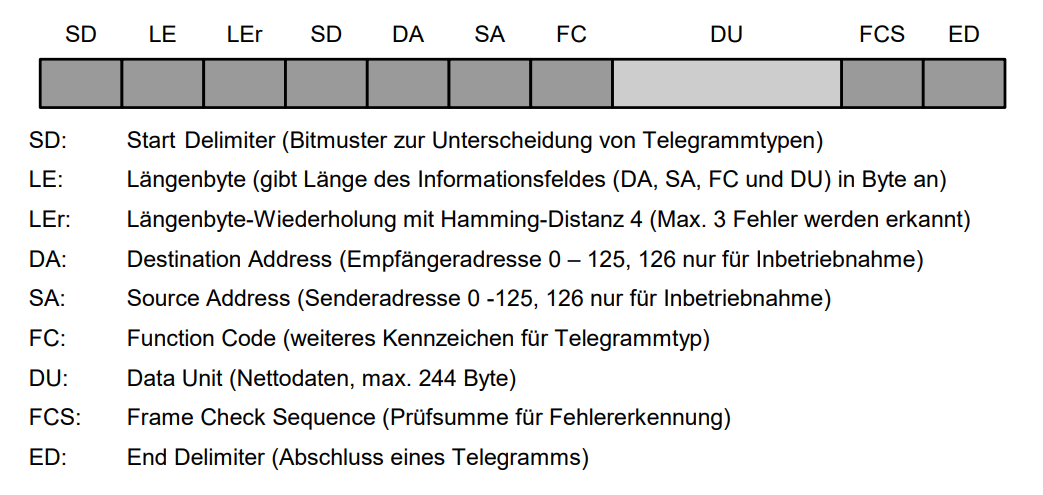
\includegraphics[width = 0.8\textwidth]{assets/img/Telegram.PNG}
               \caption{Telegrammaufbau}
        \end{center}
        \label{fig:telegramm}
        \caption{Der Aufbau eines PROFIBUS DP Telegramms}
\end{figure}

\section{Vorbereitende Arbeiten}

\section{Vorbereitung}
Zur Vorbereitung soll nun ein Grundverständnis für das bestehende Steuerungsprogramm geschaffen werden. Dazu wird das Programm in AWL analysiert und die einzelnen Schritte erklärt.

\subsection{OB100}
\label{sec:ob100}
Dieser Organisationsbaustein wird nur einmalig zur Initialisierung aufgerufen.

\begin{lstlisting}
SET
S M4.0 
L 0
T AW260
\end{lstlisting}
Hier wird der Notaus, der in der Variable \textit{M4.0} gespeichert ist, gesetzt. Dadurch ist der Notaus nicht gedrückt, da er drahtbruchsicher implementiert ist. Darüber hinaus wird die Bandgeschwindigkeit, die in AW260 ist, auf 0 gesetzt.

\subsection{OB1}
Dieser Organisationsbaustein wird zyklisch aufgerufen und ist in Netzwerke unterteilt.

\subsubsection{Netzwerk 1}

\begin{lstlisting}
  % Wenn Notaus gedrueckt ist, dann Motor aus
    UN M4.0 
    SPBN M001 
    L 0
    T AW260
    SPB M004 
M001: NOP 0
\end{lstlisting}
Dieses Netzwerk überprüft, ob der Notaus gedrückt ist. Wenn dies der Fall ist, wird der Motor ausgeschaltet. Wenn der Notaus nicht gedrückt ist, bleibt der Zustand des Motors unverändert.

\subsubsection{Netzwerk 2}

\begin{lstlisting}
  % Wenn Lichtschranke L1 unterbrochen ist, dann Motor umkehren
UN E0.2 
R A0.1
SPBN M002 
L 10000 
T AW260
M002: NOP 0
\end{lstlisting}
Dieses Netzwerk überprüft die Lichtschranke \textit{L1}. Wenn diese unterbrochen ist, wird die Drehrichtung des Motor umgekehrt, sodass das Werkstück nun wieder in Richtung der anderen Lichtschranke fährt. Wenn die Lichtschranke nicht unterbrochen ist, bleibt der Zustand des Motors unverändert. Wenn der Motor zu Anfang noch nicht gestartet war, wird die volle Drehgeschwindigkeit eingestellt und der Motor gestartet.

\subsubsection{Netzwerk 3}

\begin{lstlisting}
  % Wenn Lichtschranke L4 unterbrochen ist, dann Motor umkehren
UN E0.3
S A0.1
SPBN M003
L 10000
T AW260
M003: NOP 0
\end{lstlisting}

Dieses Netzwerk überprüft die Lichtschranke \textit{L4}. Wenn diese unterbrochen ist, wird die Drehrichtung des Motor umgekehrt, sodass das Werkstück nun wieder in Richtung der anderen Lichtschranke fährt. Wenn die Lichtschranke nicht unterbrochen ist, bleibt der Zustand des Motors unverändert. Wenn der Motor zu Anfang noch nicht gestartet war, wird die volle Drehgeschwindigkeit eingestellt und der Motor gestartet.
\subsubsection{Netzwerk 4}

\begin{lstlisting}
  %Ende des Programms
M004: NOP 0
\end{lstlisting}
Dieses Netzwerk stellt das Ende des Programms dar. Jeder Sprung zu diesem Netzwerk führt zum Ende des Programms.

\section{Aufbau}

Zunächst wird der PC gestartet und die Software \textit{TIA-Portal} gestartet. Das vorgefertigte Projekt wird geöffnet und die Variablen sowie die OBs aus der Vorbereitung hinzugefügt. Nun wird die Konfiguration getestet und das Programm auf die CPU geladen.
Sollte das Programm nun vollständig funktionieren, werden nun die folgenden Schritte zur Analyse von Telegrammen auf einem PROFIBUS DP Netzwerk durchgeführt.

\section{Aufgabe 5: Inbetriebnahme}

Die Inbetriebnahme erfolgt nun mit dem übersetzen der Steuerung und dem Starten der CPU. Legt man nun ein Werkstück in eine der beiden Lichtschranken, bewegt sich das Band in die Richtung des gegenüberliegenden Sensors. Wird das Werkstück nun in die andere Lichtschranke gelegt, bewegt sich das Band wieder in die andere Richtung. Diese Änderungen können nun über die Beobachtungstabelle eingesehen werden. Steuert man nun über diese Tabelle den Merker für den Notaus auf \textit{0}, wird die Anlage, wie gewünscht, angehalten.

\section{Aufgabe 6: ProfiTrace}

Im Folgenden sollen nun die Telegramme, die zwischen der Haupt-SPS und der dezentralen Peripherie ausgetauscht werden, untersucht werden. Startet man die ProfiTrace-Software und bekommt man von jedem Zyklus die entsprechenden Telegramme präsentiert. Jeder Zyklusdurchlauf besteht in unserem Aufbau aus dem Suchen eines zweiten Masters, die jedes Mal nicht erfolgreich ist, dann einem TokenPassing zwischen der SPS und sich selbst. Danach folgt ein Datentelegramm variabler Länge, das wie in Abbildung \ref{fig:telegramm} zu sehen ist, aufgebaut ist. Die Datenübertragung erfolgt synchron und zyklisch in einem Request/Response-Schema, bei dem die SPS ein Request an die DP schickt und die DP mit einer Response antwortet. Zum Schluss wird der Zyklus mit einer Service-Übertragung synchronisiert und beendet. Dieser Zyklus wiederholt sich nun immer wieder. (siehe Abbildung \ref{fig:profitrace})

\begin{figure}[H]
  \centering
  \label{fig:profitrace}
  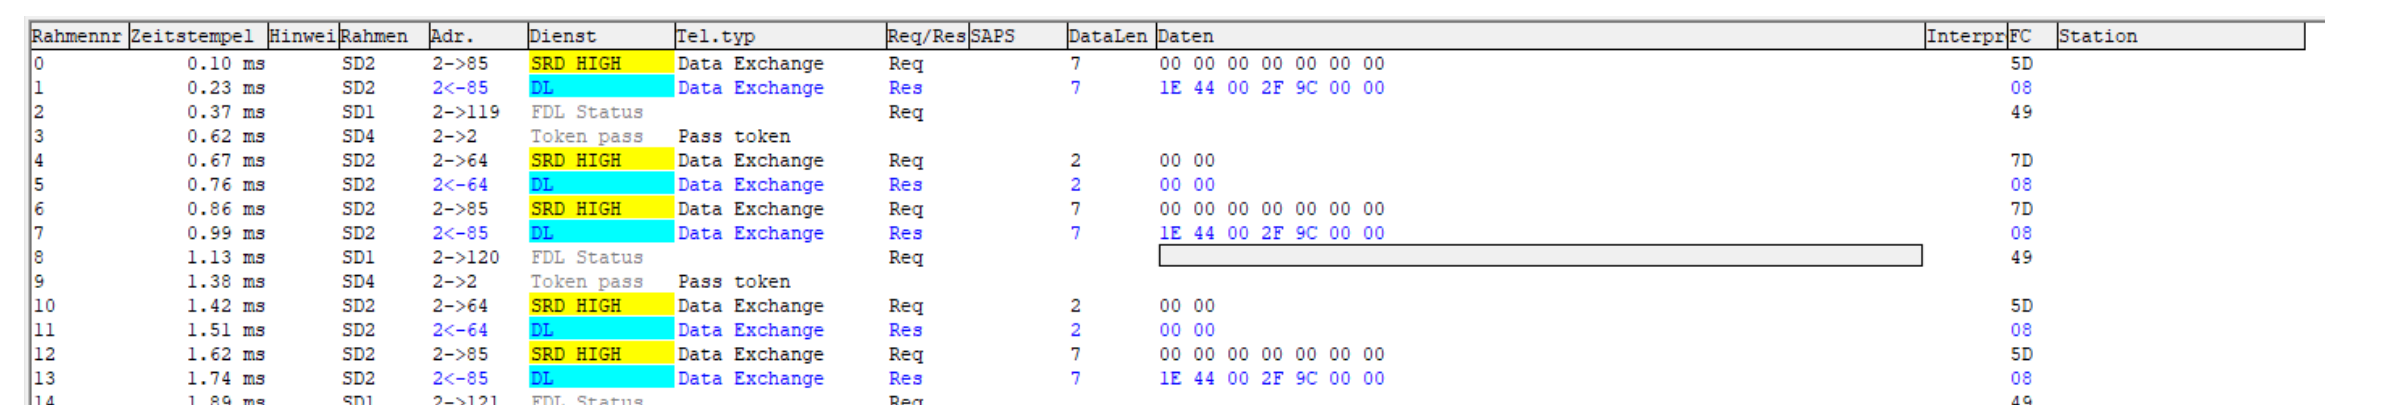
\includegraphics[width=\textwidth]{assets/img/profitrace.png}
  \caption{ProfiTrace-Ausgabe nach der Inbetriebnahme}
\end{figure}

Aus den Zeitstempeln der Telegramme lässt sich eine Zykluszeit von ungefähr $42ms$ errechnen. Das stimmt mit der voreingestellten maximalen Zykluszeit von $150ms$ überein.
Die Data Unit in den Datentelegrammen stellen Informationen und Anweisungen die von und zu der SPS fließen. Eine Änderung der Laufrichtung beispielsweise setzt andere Bits als die vorherige Richtung. Auch ein Ändern des Notauses, wie in Aufgabe 5, setzt in der Request der SPS andere Bits als im normalen Zustand. 

\section{Aufgabe 7: Busfehler}

\subsection{Aufgabe 7.1: Ausfall einer dezentralen Peripherie}

Es gibt verschieden Möglichkeiten, wie eine dezentrale Peripherie ausfallen kann. Zunächst werden wir die Adresse unseres DP-Moduls softwareseitig ändern, sodass diese nicht mehr von der SPS gefunden werden kann. Dazu wird in der Hardwarekonfiguration der SPS die Adresse des DP-Moduls geändert. Nun wird die Hardwarekonfiguration neu geladen und die SPS neu gestartet. Nun wird die SPS die dezentrale Peripherie nicht mehr finden und es wird ein Busfehler auftreten. Nach dem Korrigieren der Adresse funktioniert die Anlage wieder wie im Normalbetrieb.
Damit ein solches Problem auch außerhalb der roten LED an den Bauteilen angezeigt wird, wird nun der Ausgang A8.0 gesetzt, wenn ein Busfehler auftritt. Im OB86 folgt daher:

\begin{lstlisting}
  SET
  S A8.0
\end{lstlisting}
Der OB86 wird immer genau dann aufgerufen, wenn ein Busfehler auftritt. In diesem Fall wird nun der Ausgang A8.0 gesetzt. Im Betrieb wird dieser Vorgang nun getestet, indem der SUB-DP-Stecker bei laufender CPU gezogen wird. Es kann festgestellt werden, dass der Ausgang korrekt gesetzt wird.

\subsection{7.2: Abschlusswiderstand}

Ein Bussystem basiert stark auf ausreichende Abschlusswiderstände, die eine Reflexion der Signale am Eingang einer Baugruppe verhindern. Es wird nun simuliert, was passiert, wenn der Abschlusswiderstand in unserem Versuchsaufbau fehlt. Dazu wird der Abschlusswiderstand am SUB-D-Stecker ausgeschaltet. Durch unsere geringen Leitungslängen, funktioniert das System weiterhin fehlerfrei.

Verwendet man jedoch die Ersatzleitung, die eine Leitungslänge von ca. 150m simuliert, konnte festgestellt werden, dass die Eigenschaften des Bussystems sich drastisch ändern. Bei ausgeschaltetem Widerstand ist eine Übertragung nicht möglich und der ProfiTrace-Output besteht ausschließlich aus Fehlermeldungen. Bei eingeschaltetem Abschlusswiderstand sind die Übertragungsraten jedoch stark eingeschränkt. So ist eine Übertragung mit 12MBit/s nicht möglich, da eine höhere Übertragungsrate, genauso wie eine längere Leitungslänge Reflexionen und Interferenzen an den Bussignalen begünstigt. Es folgen inkorrekt gesetze Bytes für die korrekte Übertragung von Telegrammen und eine folgliche Lahmlegung der Kommunikation zwischen Master und Slave. Bei einer Übertragungsrate von 1,5MBit/s ist eine Übertragung jedoch möglich, da die Reflexionen und Interferenzen bei dieser Übertragungsrate nicht mehr so stark sind, dass sie die Übertragung verhindern.


\section{Aufgabe 8: Einbinden eines neuen DP-Moduls}

\subsection{Aufgabe 8.1: Einbinden ohne Hardwarekonfiguration}
Zunächst wird das neue DP-Modul an den SUB-D-Stecker angeschlossen, ohne dabei eine softwareseitige Änderung durchzuführen. Nach dem Starten wird das neuen Modul nicht gefunden und es nimmt kein direkten Einfluss auf den Programmablauf. Lediglich auf dem Busteilnehmer, der noch nicht in das System eingebunden war, wurde ein Busfehler auf der Zustands-LED angezeigt. Dieser Fehler wird durch das Fehlen der Hardwarekonfiguration verursacht.


\subsection{Aufgabe 8.2: Einbinden mit Hardwarekonfiguration}
Um nun das neue Modul in den Programmablauf einzubinden, wird zunächst über die ProfiTrace-Software das Bussystem nach neuen Teilnehmern durchsucht und die jeweilige Adresse herausgefunden. Nun kann eine Baugruppe aus dem Katalog im TIA-Portal ausgewählt werden, die mit der physischen Baugruppe übereinstimmt und in die Netzwerkübersicht gezogen. Über die Oberfläche kann nun die Verbindung zwischen den Baugruppen gezogen und die vorher ermittelte Adresse eingetragen werden. Nun kann die Hardwarekonfiguration neu geladen werden und die SPS neu gestartet werden. Nun wird das neue Modul gefunden und kann in den Programmablauf eingebunden werden.

\subsection{Aufgabe 8.3: ProfiTrace-Ausgabe}

Betrachtet man nun die ProfiTrace-Ausgabe, wird einem schnell klar, dass der Zyklus um ein Request/Response-Schema erweitert wurde. Es gibt zwar weiterhin ein Suchen nach einem zweiten Master und ein TokenPassing, aber die Datenübertragung erfolgt nun erst zu der ersten DP und dann zu der gerade neu eingebundenen DP. Die Data Unit der zweiten Peripherie ist jedoch deutlich kleiner, da es kaum Daten gibt, die übertragen werden müssen. (siehe Abbildung \ref{fig:profitrace_mehrteilnehmer})

\begin{figure}
  \centering
  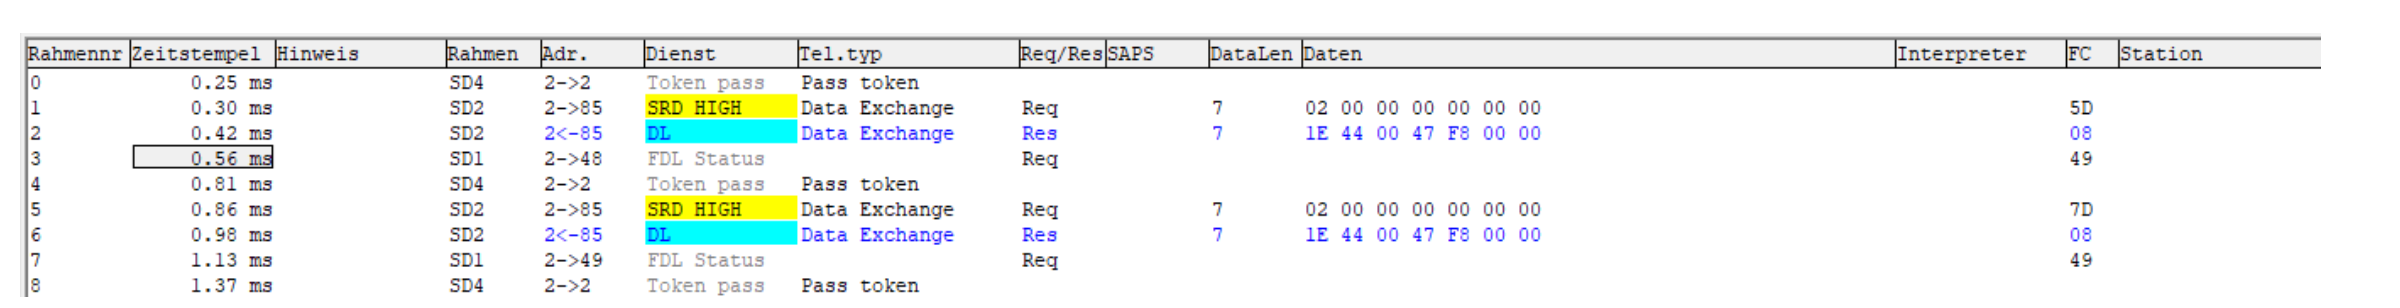
\includegraphics[width=\textwidth]{assets/img/profitrace_mehrteilnehmer.png}
  \caption{ProfiTrace-Ausgabe mit mehreren Teilnehmern}
  \label{fig:profitrace_mehrteilnehmer}
\end{figure}

\subsection{Aufgabe 8.4: Zugriff auf die Baugruppe im Programmablauf}

Um nochmal einen Zugriff auf die Baugruppe im Programmablauf zu simulieren, wird nun der Adressbereich der DP in den Einstellungen im TIA-Portal auf den Adressbereich 100 gelegt. Über die Beobachtungstabelle kann nun die Adresse 100.0 angesprochen werden. In der ProfiTrace-Software ist nun zu sehen, wie Bytes in dem Payload der Request geändert wurden. 


\section{Fazit}

Nach Abschluss des Labor lässt sich sagen, dass PROFIBUS DP mit dem richtigen Wissen und Equipment eine mächtige Technologie ist, die mit Recht in der Industrie eingesetzt wird. Es ist vergleichsweise einfach ein System aus dezentralen Peripherien aufzubauen, die gut miteinander kommunizieren um auch komplizierte Aufgaben zu lösen. Trotzdessen gibt es viele kleine Stolperfallen und das System bietet viel Platz für Optimierung, wenn man weiß, wie diese durchzuführen sind. 
Die Aufgaben haben außerdem gezeigt, dass PROFIBUS DP ein sehr robustes Bussystem ist, das auch bei fehlenden Abschlusswiderständen noch funktioniert. Es ist jedoch zu beachten, dass die Übertragungsrate bei fehlenden Abschlusswiderständen stark eingeschränkt ist.
Aus einer Software-Perspektive kann man sagen, dass das Arbeiten mit PROFIBUS DP eine auch einige Herausforderung darstellen kann, da es eine spezielle Hardware-Konfiguration erfordert und eine eigene Kommunikationsprotokoll-Schicht hat. Um mit PROFIBUS DP zu arbeiten, benötigt man eine spezielle Software, die in der Lage ist, mit dem Protokoll zu kommunizieren und die Daten zu verarbeiten. Es gibt jedoch auch Bibliotheken und Frameworks, die die Arbeit mit PROFIBUS DP erleichtern können. In der Regel müssen Entwickler auch über Kenntnisse in der Automatisierungstechnik verfügen, um die Anforderungen der Anlage und die Kommunikation mit der SPS zu verstehen.

\end{document}
